% Website figure based on the checker game of:
%   Ravi Vakil, "A geometric Littlewood-Richardson rule",
%   Annals of Mathematics 164 (2006), 371-422. arXiv:math/0302294.
%
% Vakil's figures are xfig/epic pictures, not TikZ; this is an original TikZ
% redraw of one move from his Fig. "Two checker games with the same starting
% position" (g24): G(2,4), A = B = {2,4}, i.e. the class of a point-line
% incidence squared. Conventions follow the paper: rows are numbered from the
% top and columns from the left; black checkers encode the relative position
% of the two flags, white checkers the moving 2-plane.
%
% The move shown: the black checker in row 2 descends and the one in row 3
% rises. The critical row (row 2, from the descending checker rightwards) holds
% a white checker, and so does the critical diagonal (from the rising checker
% down-right) away from the rising checker's square, with no blocker between
% them -- the central case of Vakil's Phase 1 table, "swap or stay". So the
% degeneration breaks into two components: staying leads to the output {2,3},
% swapping (then the Phase 2 slide) to {1,4}; together
%   sigma_1^2 = sigma_{1,1} + sigma_2 in H^*(G(2,4)).
% See the publication for the original figure's rights.

\documentclass[tikz,border=4pt]{standalone}
\usepackage{amssymb}
\usetikzlibrary{arrows.meta,calc}

\definecolor{paper}{HTML}{F7F5F0}
\definecolor{ink}{HTML}{18202A}
\definecolor{muted}{HTML}{65707A}
\definecolor{line}{HTML}{D9D6CE}
\definecolor{accent}{HTML}{1C5A76}
\definecolor{accentdark}{HTML}{123D51}
\definecolor{critred}{HTML}{B5473A}
\definecolor{ochre}{HTML}{C8962E}

\newcommand{\cell}{0.42}

% square (r,c) in board-local coordinates: row r from the top, column c from the left
\newcommand{\sq}[2]{({(#2-0.5)*\cell},{-(#1-0.5)*\cell})}

% \board{name}{x}{y}: 4x4 grid with its top-left corner at (x,y)
\newcommand{\board}[3]{%
  \begin{scope}[shift={(#2,#3)}, name prefix=#1-]
    \coordinate (nw) at (0,0);
    \coordinate (se) at ({4*\cell},{-4*\cell});
    \coordinate (w)  at (0,{-2*\cell});
    \coordinate (e)  at ({4*\cell},{-2*\cell});
    \draw[ink, line width=.45pt] (0,0) grid[step=\cell] ({4*\cell},{-4*\cell});
  \end{scope}}

% checkers; a black and a white checker sharing a square are offset, as in Vakil's figures
\newcommand{\B}[4]{\begin{scope}[shift={(#1,#2)}]\fill[ink] \sq{#3}{#4} circle (0.14);\end{scope}}
\newcommand{\W}[4]{\begin{scope}[shift={(#1,#2)}]\draw[ink, line width=.6pt, fill=white] \sq{#3}{#4} circle (0.14);\end{scope}}
\newcommand{\BW}[4]{\begin{scope}[shift={(#1,#2)}]
  \fill[ink] \sq{#3}{#4} ++(-0.045,0.045) circle (0.125);
  \draw[ink, line width=.6pt, fill=white] \sq{#3}{#4} ++(0.06,-0.06) circle (0.125);\end{scope}}

\begin{document}
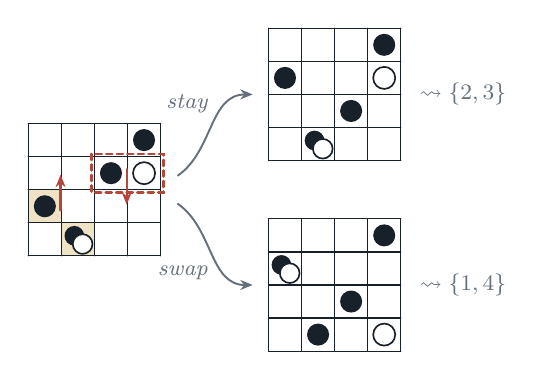
\begin{tikzpicture}[>={Stealth[length=4.5pt,width=3.6pt]}, line cap=round]

% ================= before the move =================
\def\bx{0} \def\by{0.84}
% critical diagonal: from the rising checker's square (3,1) down-right
\begin{scope}[shift={(\bx,\by)}]
  \foreach \r/\c in {3/1, 4/2}
    \fill[ochre, opacity=.28] ({(\c-1)*\cell},{-(\r-1)*\cell}) rectangle ++(\cell,-\cell);
\end{scope}
\board{A}{\bx}{\by}
% critical row: row 2, from the descending checker's column to the right edge
\begin{scope}[shift={(\bx,\by)}]
  \draw[critred, line width=.9pt, dash pattern=on 2.2pt off 1.6pt]
    ({2*\cell-0.035},{-\cell+0.035}) rectangle ({4*\cell+0.035},{-2*\cell-0.035});
\end{scope}
\B{\bx}{\by}{1}{4}
\B{\bx}{\by}{2}{3}
\B{\bx}{\by}{3}{1}
\W{\bx}{\by}{2}{4}
\BW{\bx}{\by}{4}{2}
% descending and rising checkers
\begin{scope}[shift={(\bx,\by)}]
  \draw[->, critred, line width=.85pt] ({2.5*\cell+0.2},{-1.5*\cell+0.05}) -- ({2.5*\cell+0.2},{-2.5*\cell+0.02});
  \draw[->, critred, line width=.85pt] ({0.5*\cell+0.2},{-2.5*\cell-0.05}) -- ({0.5*\cell+0.2},{-1.5*\cell-0.02});
\end{scope}

% ================= the two possible outcomes =================
\def\sx{3.05} \def\sy{2.05}   % stay
\def\wx{3.05} \def\wy{-0.37}  % swap

\board{S}{\sx}{\sy}
% stay: the white checkers keep their squares (2,4) and (4,2)
\B{\sx}{\sy}{1}{4}
\B{\sx}{\sy}{2}{1}
\B{\sx}{\sy}{3}{3}
\BW{\sx}{\sy}{4}{2}
\W{\sx}{\sy}{2}{4}

% swap: rows exchanged to (4,4) and (2,2); Phase 2 slides (2,2) left to (2,1)
\board{W}{\wx}{\wy}
\B{\wx}{\wy}{1}{4}
\BW{\wx}{\wy}{2}{1}
\B{\wx}{\wy}{3}{3}
\B{\wx}{\wy}{4}{2}
\W{\wx}{\wy}{4}{4}

% ================= arrows =================
\draw[->, muted, line width=.7pt] (A-e) ++(0.22,0.18) to[out=35,in=180] node[pos=.55, above left=-1pt, font=\footnotesize\itshape, muted] {stay} ($(S-w)+(-0.2,0)$);
\draw[->, muted, line width=.7pt] (A-e) ++(0.22,-0.18) to[out=-35,in=180] node[pos=.55, below left=-1pt, font=\footnotesize\itshape, muted] {swap} ($(W-w)+(-0.2,0)$);

% where each branch ends (the rest of Vakil's two games)
\node[anchor=west, muted, font=\footnotesize] at ($(S-e)+(0.12,0)$) {$\rightsquigarrow\{2,3\}$};
\node[anchor=west, muted, font=\footnotesize] at ($(W-e)+(0.12,0)$) {$\rightsquigarrow\{1,4\}$};

\end{tikzpicture}
\end{document}
